\section{Introduction}
\label{sec:intro}

Real-world distributed programs are challenging to write and maintain
because they often conflate two distinct mechanisms.  The first
concerns the expression of application logic - how do we define
computations that are robust in the presence of distributed
communication among concurrently executing threads of control?  The
second deals with system concerns - how do we express notions of
visibility, replication, and consistency when the nodes participating
in such computations may be geographically distributed and the
networks that connect them unreliable?  To simplify reasoning in such
complicated environments, programming models often make strong
assumptions on the guarantees provided by an implementation (such as
serializability~\cite{Serializability} or strong
consistency~\cite{CDE+12,DNN+15}) that may inadvertently mask,
restrict, or ignore important albeit unpleasant realities (e.g.,
network partitions~\cite{Brewer2000,Gilbert2002}). When unwarranted
assumptions are made, program behavior is often difficult to predict
and verify.  On the other hand, when these features are explicitly
exposed to the programmer, e.g., by requiring that applications be
written in terms of specialized distributed data
structures~\cite{Burckhardt2014,BFL+12,SPB+11} or control
primitives~\cite{Calm}, simplicity, composability, and
ease-of-reasoning can suffer.

In this paper, we consider how declarative abstractions can be used to
overcome this tension to provide the best of both worlds: functional
programs whose logical structure can be seamlessly transplanted to a
distributed setting, while nonetheless being resilient to system
realities such as network failure and latency.  Our key insight is the
development of a principled methodology that allows us transform
low-level operational details such as replication and consistency
into high-level compositional reasoning on language-level datatypes.

To illustrate how the kinds of problems described above manifest in
practice, consider how we might write a simple counter library (see
Fig.~\ref{fig:counter-adt}).  A \C{Counter} supports two (update)
operations - \C{add} and \C{mult} - that lets a non-negative integer
value be added or multiplied to the counter, resp.  Observe that the
library is written in an idiomatic functional style, with no special
reasoning principles needed to realize desired functionality.  As long
as applications use the library on a single machine, this
implementation behaves as expected.  However, if the library is used
in the context of a more sophisticated application, say one whose
computation is distributed among a collection of machines, its
behavior can become significantly harder to understand.  In
particular, a distributed implementation might wish to
\emph{replicate} the counter state on each node to improve response
time or fault tolerance.  Unfortunately, adding replication doesn't
come for free.  Attempting to update every replicated copy atomically
is problematic in the absence of sophisticated transaction support,
which impose significant performance penalties.  But, without such
heavyweight mechanisms, applying an \C{Add} operation on one node may
not be instantaneously witnessed on another, which may be in the
process of simultaneously attempting to perform its own \C{Add} or
\C{Mult} action.  While synchronizing the activities of all nodes to
ensure at most one such operation is performed at a time is
impractical, designating a single node to hold the counter state
eschewing replication altogether (as in a client-server
configuration~\cite{Armstrong}), is also an undesirable solution,
given the sensitivity of such architectures to network partitions and
server failures, and the negative performance impact it incurs in
geo-distributed environments~\cite{Walter}.  Removing coordination
altogether by simply replicating counter state without having any
supporting consistency protocol is an equally infeasible approach.

A method often adopted to address these concerns is to re-define a
datatype's operations to return \emph{effects} instead of
values~\cite{SPB+11,Burckhardt2014}.  An \emph{effect} is a tag that
identifies the operation to be applied uniformly at all replicas to
incorporate the effects of the original
operation. Fig.~\ref{fig:counter-rdt} shows the \C{Counter} library
with operations re-defined to returns effects.  Observe that the
\C{Counter.add x v} operation now returns an \C{Add x} effect, which,
when applied at a replica (see \C{apply} in the figure), adds \C{x} to
the local counter value.  Note, however, that \C{add} and \C{mult} are
not commutative operations - assuming two replicas have the same
initial counter value of 0, applying the effect of adding 3 and then
multiplying 5 on one replica yields 15, while applying the effect of
first multiplying 5 and then adding 3 yields 3 on the other.  Such
scenarios are possible in a distributed system because there are no
coherence guarantees on the order in which effects are received by
different nodes.  Thus, implementations must be carefully written to
take the lack of commutativity into account when defining how effects
are applied at a replica; in the figure, multiplication is expressed
in terms of addition to avoid the kind of undesirable behavior
described above.

In this implementation, all replicas will eventually contain the same
counter value, assuming updates to the counter eventually quiesces.
While transmitting effects provide a low-level operational basis for
handling replicated state, the \emph{ad hoc} nature of the solution
confounds desirable high-level reasoning principles.  Indeed, the
semantic gap between the two versions of the counter, one cognizant of
replication and the other not, breaks backward compatibility with the
original state-based implementation.  Just as significantly, its
non-trivial construction must be developed in different guises for
every distributed data structure used by the application.
\begin{figure}
\begin{subfigure}[b]{0.4\textwidth}
  \begin{ocaml}
    module Counter: sig
      type t
      val add: int -> t -> t
      val mult: int -> t -> t
      val read: t -> int
    end = struct
      type t = int
      let add x v = v + (abs x)
      let mult x v = v * (abs x)
      let read v = v
    end
  \end{ocaml}
\caption{\C{Counter} library in OCaml}
\label{fig:counter-adt}
\end{subfigure}
\begin{subfigure}[b]{0.56\textwidth}
  \begin{ocaml}
    module Counter: sig
      type t
      type eff
      val add: int -> t-> eff
      val mult: int -> t -> eff
      val apply: eff -> t -> t
      val read: t -> int
    end = struct
      type t = int
      type eff = Add of int
      let add x v = Add (abs x)
      let mult x v = Add (v * (abs x - 1))
      let apply (Add x) v = x + v
      let read v = v
    end
  \end{ocaml}
\caption{\C{Counter} library re-engineered for effect-based replication}
\label{fig:counter-rdt}
\end{subfigure}
\end{figure}
The lack of composability is yet another important downside of this
approach.  Consider an application that uses two replicated counters,
$c_1$ and $c_2$, bound by the invariant $c_2 \ge c_1$, duly enforced
by the application when updating $c_2$ or $c_1$.  An execution may
nonetheless witness anomalous states that violate the invariant
because updates to $c_1$ and $c_2$ may be applied independently in any
order on any replica.  For example, if a replica increments both
counters, a \C{read} operation performed at another replica may
\begin{wrapfigure}{L}{.5\textwidth}
  \begin{center}
    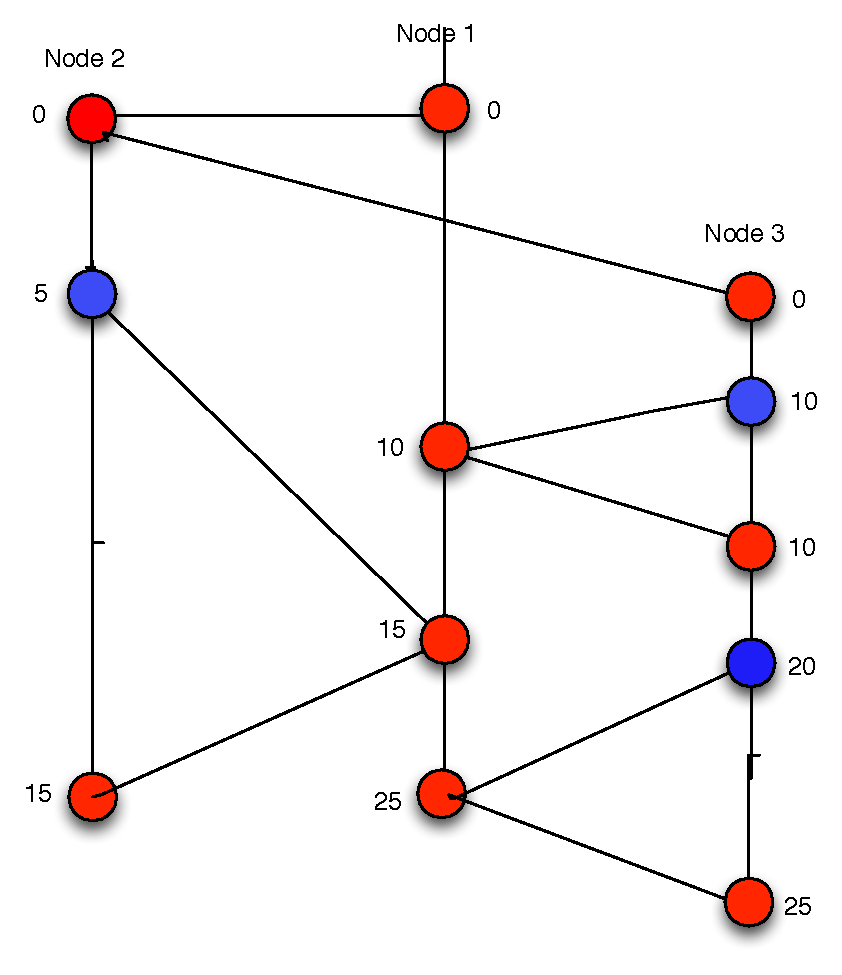
\includegraphics[scale=0.4]{Figures/dali-counter}
  \end{center}
  \caption{\small A replicated counter can be expressed as a sequence
    of versions managed by logically-distributed concurrently
    executing threads.  Local versions produced by these threads
    periodically merge their state with one another.  In the figure,
    when the local version of Node 3, labeled 20, merges with the
    local version of Node 1, whose counter state is 15 at the time, a
    new counter value is produced.  This value takes into account the
    previous merged state (10) from which the two versions were
    derived to yield a new merged state of 25.  There is no other form
    of synchronization or coordination among versions except through
    merging.  In the figure, red circles represent counter state
    produced through merging, and blue circles represent state
    produced by applying counter operations on a node-local version.
  }
	\vspace*{-1.2in}
\end{wrapfigure}
witness the increment to $c_1$, but not $c_2$, thus violating the
invariant. The intention to atomically apply both effects cannot be
captured in the absence of external mechanisms to compose effects
(such as effect-based transactions~\cite{pldi15}).  Rather than
viewing a distributed computation in terms of \C{Add} effects produced
by operations, can we formulate a more declarative interpretation,
directly in terms of the counter value maintained by each node?  To do
so, we first observe that each replica essentially operates over its
own version of a counter.  Thus, local operations on a replicated
object can be thought of as yielding new versions, collectively
producing a version tree, with one branch for each replica.  Every
branch represents different (immutable) versions maintained by
different nodes, with the state produced by the computation performed
over a counter on a node recorded along the node's local branch for
the counter.  Now, to generate a globally consistent view of a
counter, we only need to define a merge operation that explains how to
combine two local versions to produce a new version that reflects both
their states.  This operation is defined not in terms of replicas or
other system-specific artifacts, but in terms of the semantics of the
datatype itself.

Framing replication as merging leads to a counter implementation that
bears strong similarity to the original sequential one:
  \begin{ocaml}
    module Replicated_Counter = struct
      include Counter
      let merge lca v1 v2 =
         lca + (v1 - lca) + (v2 - lca)
    end
  \end{ocaml}
The role of \C{lca} (lowest common ancestor) here captures salient
history - the state resulting from the merge of two versions derived
from the same ancestor state should not unwittingly duplicate the
contributions of the ancestor.  This interpretation of a replicated
datatype is thus given in terms of the evolution of a program state
implicitly associated with the different nodes that comprise a
distributed application with merge operations serving to communicate
and reconcile different local states.

Our main innovation is thus the development of a programming model
that realizes a monadic version control system centered around data,
rather than file, coherence.  The \name monad lets programmers write
and compose concurrent computations around multiple (implicit)
versions of a mergeable datatype, an ordinary ML datatype additionally
equipped with a \emph{merge} function responsible for deriving a
consistent global state from a collection of local versions of that
state.  A computation progresses by forking (i.e., replicating) new
versions of existing versions, allowing synchronization-free local
computation to proceed on those nodes, creating new versions along an
existing \emph{branch} that represents updated local instances, and by
merging branches to realize global consistency.

Our model allows ML programmers to get the benefits of achieving
highly available (low-latency) distributed computation, while
continuing to enjoy the comforts of high-level reasoning and the
familiarity of using standard libraries already provided by the
language.  Notably, while \name's programming model makes no explicit
reference to any specific operational manifestation of a distributed
system (e.g., programmers do not need to explicitly manage replicas),
we demonstrate that it can be nonetheless efficiently realized on
existing real-world geo-replicated distributed systems.

Our contributions are summarized below:

\begin{itemize}
    \item We formally introduce the concept of a \emph{mergeable}
      datatype to admit high-level declarative reasoning about
      distributed computation and replicated state in ML programs.

    \item We describe \name programming model that brings to bear the
      power and flexibility of a version control system to the
      administration of replicated data. \name hides the complexity of
      version control behind a monad, and exposes its functionality
      via a simple API that lets programmers define and compose
      distributed ML computations around such data.  Issues related to
      replication only manifest implicitly in the definition of a
      merge operation that defines coherence among different instances
      of replicated state.

    \item We present a formalization of the \name programming model,
      and establish the conditions under which eventual convergence of
      concurrent version state can be guaranteed.

    \item We describe an implementation of the \name library that
      transparently adds persistence and replication features to a
      mergeable type, and which sits atop the Irmin persistent
      store~\cite{irmin}, a content-addressable storage library for
      OCaml. We also present case studies and experimental results
      that justify the practical utility of our approach.
\end{itemize}

\noindent The remainder of the paper is organized as follows.  We present the
\name\ programming model informally in the next section.
Sec.~\ref{sec:mergeable_types} develops a series of examples that
illustrate how merge operations can be defined and used.
Sec.~\ref{sec:formalization} defines an operational semantics, and
formalizes our intuition of a mergeable type in terms of morphisms over
datatype operations.  We also present soundness (consistency) and
progress guarantees enjoyed by the
semantics. Sec.~\ref{sec:system-model} considers an instantiation of
the model suitable for distributed environments with network
partitions and failures.  Implementation details describing how we
incorporate mergeable types into OCaml are presented in
Sec.~\ref{sec:impl}.  Experimental results and benchmarks are given in
Sec.~\ref{sec:evaluation}.  Secs.~\ref{sec:related}
and~\ref{sec:conclusions} describes related work and conclusions.


%% Persistence adds yet another dimension to the problem. Functional data
%% structures are often large in-memory linked structures that admit
%% functional updates by creating newer versions that share most of their
%% structure with previous versions. Sharing is the key to efficiency,
%% without which every functional update takes time that is at least
%% linear in the size of the data structure. Unfortunately, the
%% straightforward way to persist a data structure on disk in a
%% machine-agnostic format (e.g., JSON) requires serialization, which is
%% linear in the size of the data structure. An alternative is to
%% maintain a separate on-disk copy of the data and administer it via a
%% database system. The downside is that the programmer is now required
%% to reason in terms of a lower-level abstraction (e.g., a relational
%% data model) in order to maintain coherence between in-memory and
%% on-disk representations. Safety guarantees over the in-memory data do
%% not carry over to the disk, which introduces additional complications
%% and the possibility of new bugs. Thus, adding persistence to
%% applications while preserving high-level safety gurantees offered by
%% the language abstraction is a non-trivial problem.



%% However, as we shall see,
%% unconstrained branching may yield a branching structure that becomes
%% unmergeable, thus leading to \emph{stuck} states. An important
%% property of the \name library is that it guarantees progress even in
%% the presence of arbitrary merges provided the merge operation is
%% commutative with respect to its version state arguments.  Furthermore,
%% \name profitably exploits provenance information available via
%% branches to make application resilient to network partitions.
%% In this paper, we define a semantics of mergeable datatypes that lets
%% any OCaml program be seamlessly deployed in a distributed environment
%% with implicit support for replicated and decentralized operation.  The
%% underlying foundation for merge actions has a natural category
%% theoretic interpretation that enables us to construct useful mergeable
%% variants for \emph{any} OCaml type whose states are commutative wtih
%% respect to the merge operation defie
